% -*- coding: utf-8 -*-
% 2 ページ版（A4・2 段組）。8 ページ版 tr_cad.tex の要約。
% コンパイル: lualatex tr_cad_2p.tex （2 回）
%
% 体裁は講演会論文の一般的な形（和文題目＋英文題目＋英文 Abstract＋Key Words）に
% 寄せてあるが、特定の学会の様式ではない。
\documentclass[a4paper,9pt,twocolumn]{ltjsarticle}

\usepackage{luatexja-fontspec}
\usepackage[top=20mm,bottom=20mm,left=20mm,right=20mm,columnsep=8mm]{geometry}
\usepackage{graphicx}
\usepackage{booktabs}
\usepackage{amsmath}
\usepackage{caption}
\usepackage{float}
\usepackage{enumitem}
\usepackage[hidelinks]{hyperref}
\usepackage{url}

\captionsetup{font=footnotesize,labelfont=sc,skip=3pt}
\captionsetup[table]{position=top}
\setlist{itemsep=0pt,topsep=2pt,parsep=0pt,leftmargin=1.5em}
\renewcommand{\arraystretch}{1.05}
\newcommand{\code}[1]{\texttt{\scriptsize #1}}
% ⚠ 単位は立体。数式中で \mm と書くと mm が数式イタリックになるので \mathrm で囲む。
\newcommand{\mm}{\ensuremath{\,\mathrm{mm}}}
\pagestyle{empty}
% ⚠ 図 4 点・表 2 点を 2 ページに収めるため、フロートまわりの余白を詰める
\setlength{\textfloatsep}{6pt plus 2pt minus 2pt}
\setlength{\floatsep}{5pt plus 2pt minus 2pt}
\setlength{\intextsep}{5pt plus 2pt minus 2pt}
\setlength{\dblfloatsep}{5pt plus 2pt minus 2pt}
\setlength{\dbltextfloatsep}{6pt plus 2pt minus 2pt}
\setlength{\abovedisplayskip}{3pt}
\setlength{\belowdisplayskip}{3pt}

\begin{document}
\twocolumn[
\begin{@twocolumnfalse}
\begin{flushright}\footnotesize 2026 年 8 月\end{flushright}
\vspace{-2mm}
\begin{center}
{\large\bfseries 検査駆動によるパラメトリック CAD 設計法}\\
\vspace{1mm}
{\normalsize 競技ロボットの機体設計における設計妥当性の自動判定と，その失敗様式の類型化}\\
\vspace{2mm}
{\normalsize Inspection-Driven Parametric CAD Design}\\
{\footnotesize Automated Design Validation and a Taxonomy of Its Failure Modes
in Competition Robot Development}\\
\vspace{2mm}
{\normalsize 貝淵 蒼馬}
\end{center}
\vspace{1mm}

\begin{center}\vspace{-2mm}
\begin{minipage}{0.93\textwidth}
\footnotesize
\textit{Abstract}: In short-term robot development, CAD is used as a drawing tool
and design validity is usually discovered by hand during assembly.
This paper reports an inspection-driven design method in which geometry, joints,
mass and manufacturing data are all generated from a single parametric source,
and design validity is judged by 34 automated inspections instead of visual review.
Fastening relations are held as declarations rather than inferred from geometry,
plate outlines are determined by SIMP topology optimization whose boundary
conditions are generated from those declarations, and fastener positions are
frozen from solid point-membership tests to break the circular dependency
between assembly and placement.
Applied to a 1,224-solid competition robot, the method detected defects that were
invisible on drawings, including five geometrically unassemblable interferences,
a mounting declaration with zero bearing area, and pilot holes breaking through
the side wall of a 6 mm rib by 0.25 mm.
The observed defects are organized into six failure modes; in particular,
an inspection is shown to be trustworthy only after it has been verified to fail
on a deliberately injected defect.

\vspace{1.2mm}
\noindent\textit{Key Words}: Design automation, Parametric CAD, Topology optimization,
Interference inspection, Robot contest

\vspace{1.2mm}
\noindent\textbf{公開データ}\quad STEP・URDF・製作データ:
\url{https://github.com/Raptor-zip/NHK-K2026/releases/tag/cad-v1.0}
／ 全 12 関節を動かせるビューア:
\url{https://3d-view.raptor-s.workers.dev/?model=/local/nhk-tr/tr.urdf}
\end{minipage}\vspace{-3mm}
\end{center}
\vspace{2mm}
\end{@twocolumnfalse}
]

%----------------------------------------------------------------------
\section{緒言}

競技ロボットの機体開発は期間が短く，設計者も少ない。
この条件下では CAD は「形を描く道具」として用いられ，
干渉・締結・質量・加工性の妥当性は図面の目視と組立時の発見に委ねられる。
反復のコストが物理的であり，一つの見落としが数日の手戻りに直結する。

本研究では，これに対する構成的な代替として次の四原則からなる設計法を構築し，
実機規模の競技ロボット（ソリッド 1{,}224，可動関節 12，アクチュエータ 11 軸，
外形 $964\times803\times1191\mm$）に適用した。
(i) 形状はコードで生成し寸法の情報源を単一化する，
(ii) 固定関係を幾何から推定せず宣言として保持する，
(iii) 妥当性は宣言と実体を突き合わせる自動検査が判定する，
(iv) 検出できなかった不良が出たら部品ではなく検査を改修する。

本稿の主たる貢献は個々の機構設計ではなく，
適用過程で観測された不良を六つの様式に類型化した点にある。

%----------------------------------------------------------------------
\section{設計法}

\subsection{固定関係の宣言的記述}

部品配置時に，固定先・留め方・員数と規格を明示的に与える。
留め方はボルト，溝ナット，リベット，溶接，圧入，回転対偶，滑り対偶，
載置，挟持，縫合，調整代など 20 種以上を区別する。
この宣言により，浮き（どこにも固定されていない），離れ（固定先と接していない），
宣言のない接触，許容を超える干渉，座面積の不足，リンクを跨ぐ不正な締結が，
幾何から機械的に判定できる。

判定基準を距離から宣言へ移したことが要点である。
距離基準では「偶然近接している」ことと「固定されている」ことが区別できない。
市販 CAD の干渉チェックが判定できるのは前者までであり，
本手法は意図を宣言として保持することで後者を判定対象に置く。

\subsection{境界条件を宣言から生成する位相最適化}

構造板の外形は，四節点平面応力要素による有限要素解析と SIMP 法で決定する。
境界条件は手書きせず，固定宣言の向きから生成する。
すなわち，当該板が固定されている相手を拘束，
当該板に固定されている相手を荷重，
締結の座面を密度 1 の保存領域，
板を貫通する相手を密度 0 の除去領域として与える（図\ref{fig:topo}）。
13 枚の適用で $1.62\,$kg を削減した（図\ref{fig:heat}）。

\subsection{凍結生成物と収束}

組立モデルを読んでから決まる生成物が二つある。
締結要素の位置と，板の最適化輪郭である。
前者は板の外形から座面を探索し，後者は締結の座面を保存領域として解くため，
両者は相互依存し不動点をなす。一巡では不整合が残り，二巡で収束する。
鮮度判定にはファイル更新時刻を用いず，境界条件と部品形状の指紋を用いる。

%----------------------------------------------------------------------
\begin{figure*}[t]
\centering
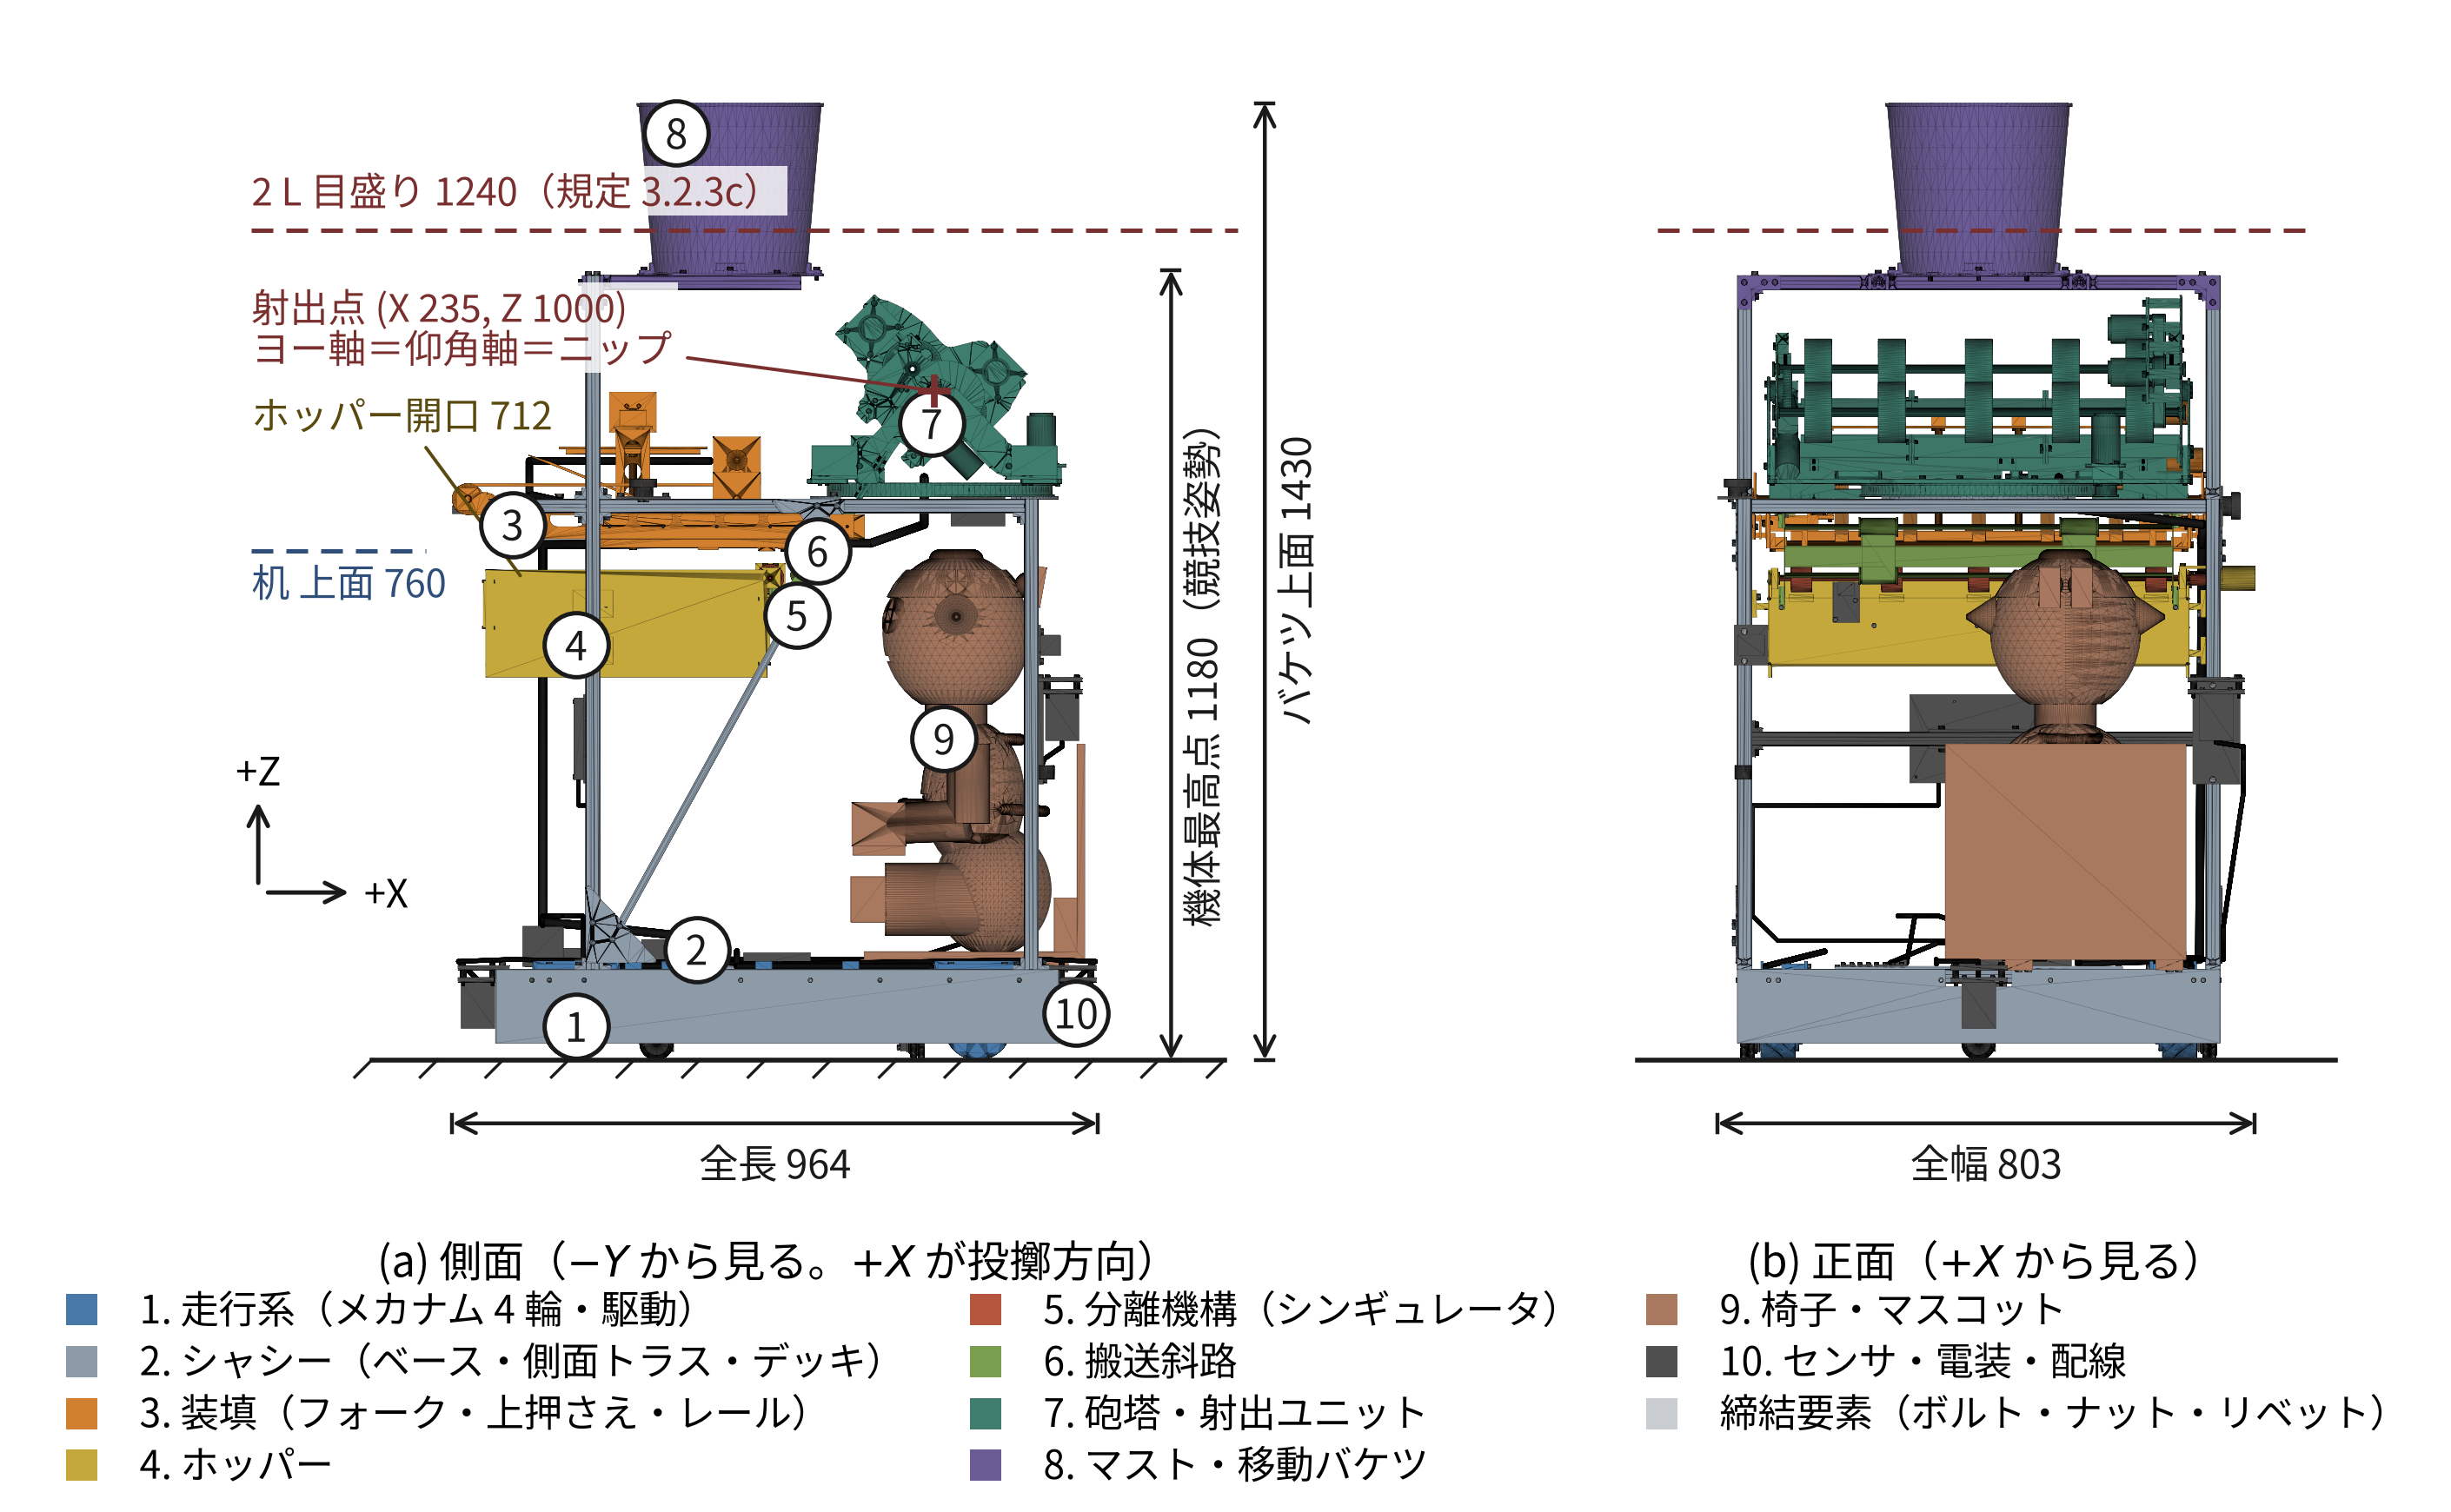
\includegraphics[width=0.66\textwidth]{figs/fig1.png}
\caption{対象機体（競技姿勢）。組立モデルの三角メッシュを正射影し，
面法線の奥行成分で陰影を与えた。色は系統，白丸の番号は凡例に対応する。
寸法・基準線はすべて組立から実測しており，図中に手入力した数値はない。
$2\,$L 目盛りの破線は機体の高さの上限（規定 3.2.3c）で，搭載バケツ自体は対象外である。}
\label{fig:match}
\end{figure*}

%----------------------------------------------------------------------
\section{適用結果}

最終形は表\ref{tab:result}のとおりで，質量を除き規定に適合する。
干渉検査は 3 姿勢 $\times$ 17 ペアで適合，
組立検査は浮き・分断・リンク跨ぎ・座面不足のいずれも 0 である。
製作データとして切抜 140 点，3D 造形 31 点を出力できる。

\begin{table}[t]
\centering\footnotesize
\caption{規定適合の自動判定（抜粋）}
\label{tab:result}
\begin{tabular}{@{}lrrl@{}}
\toprule
項目 [mm, kg] & 設計値 & 規定 & 判定\\
\midrule
スタート時外形 & $964\times803\times1191$ & $\le1000\times1000\times1200$ & 適合\\
競技中最大展開 & $1189\times803\times1191$ & $\le1200\times1200\times1800$ & 適合\\
フォーク実形状最下点 & 760.50 & $760.5$--$762$ & 適合\\
質量 & 39.08 & $\le35.0$ & 不適合\\
\bottomrule
\end{tabular}
\end{table}

本手法は，図面上では認識できない不良を検出した。
可動部が固定部を貫通する組立不能な形状 5 件，座面積が零の取付宣言，
下穴が板厚 $6\mm$ の耳の側面を $0.25\mm$ 破る締結配置，
線形従属な計測輪配置による横速度の不可観測性などである。
また，概算 $0.70\,$kg としていた締結具質量が実測 $3\,$kg 超であることが判明し，
規定質量の超過が顕在化した。

静的な検査に加え，生成した URDF を物理エンジンに読み込み，
競技環境を配置して機構シミュレーションを行い，
図面では検出できない 9 件の不具合を検出した。
たとえば，引込後に布を移送する手段が存在しない事象であり，
カム駆動の受動関節を追加してアクチュエータを増やさずに解決した。

%----------------------------------------------------------------------
\begin{figure}[b]
\centering
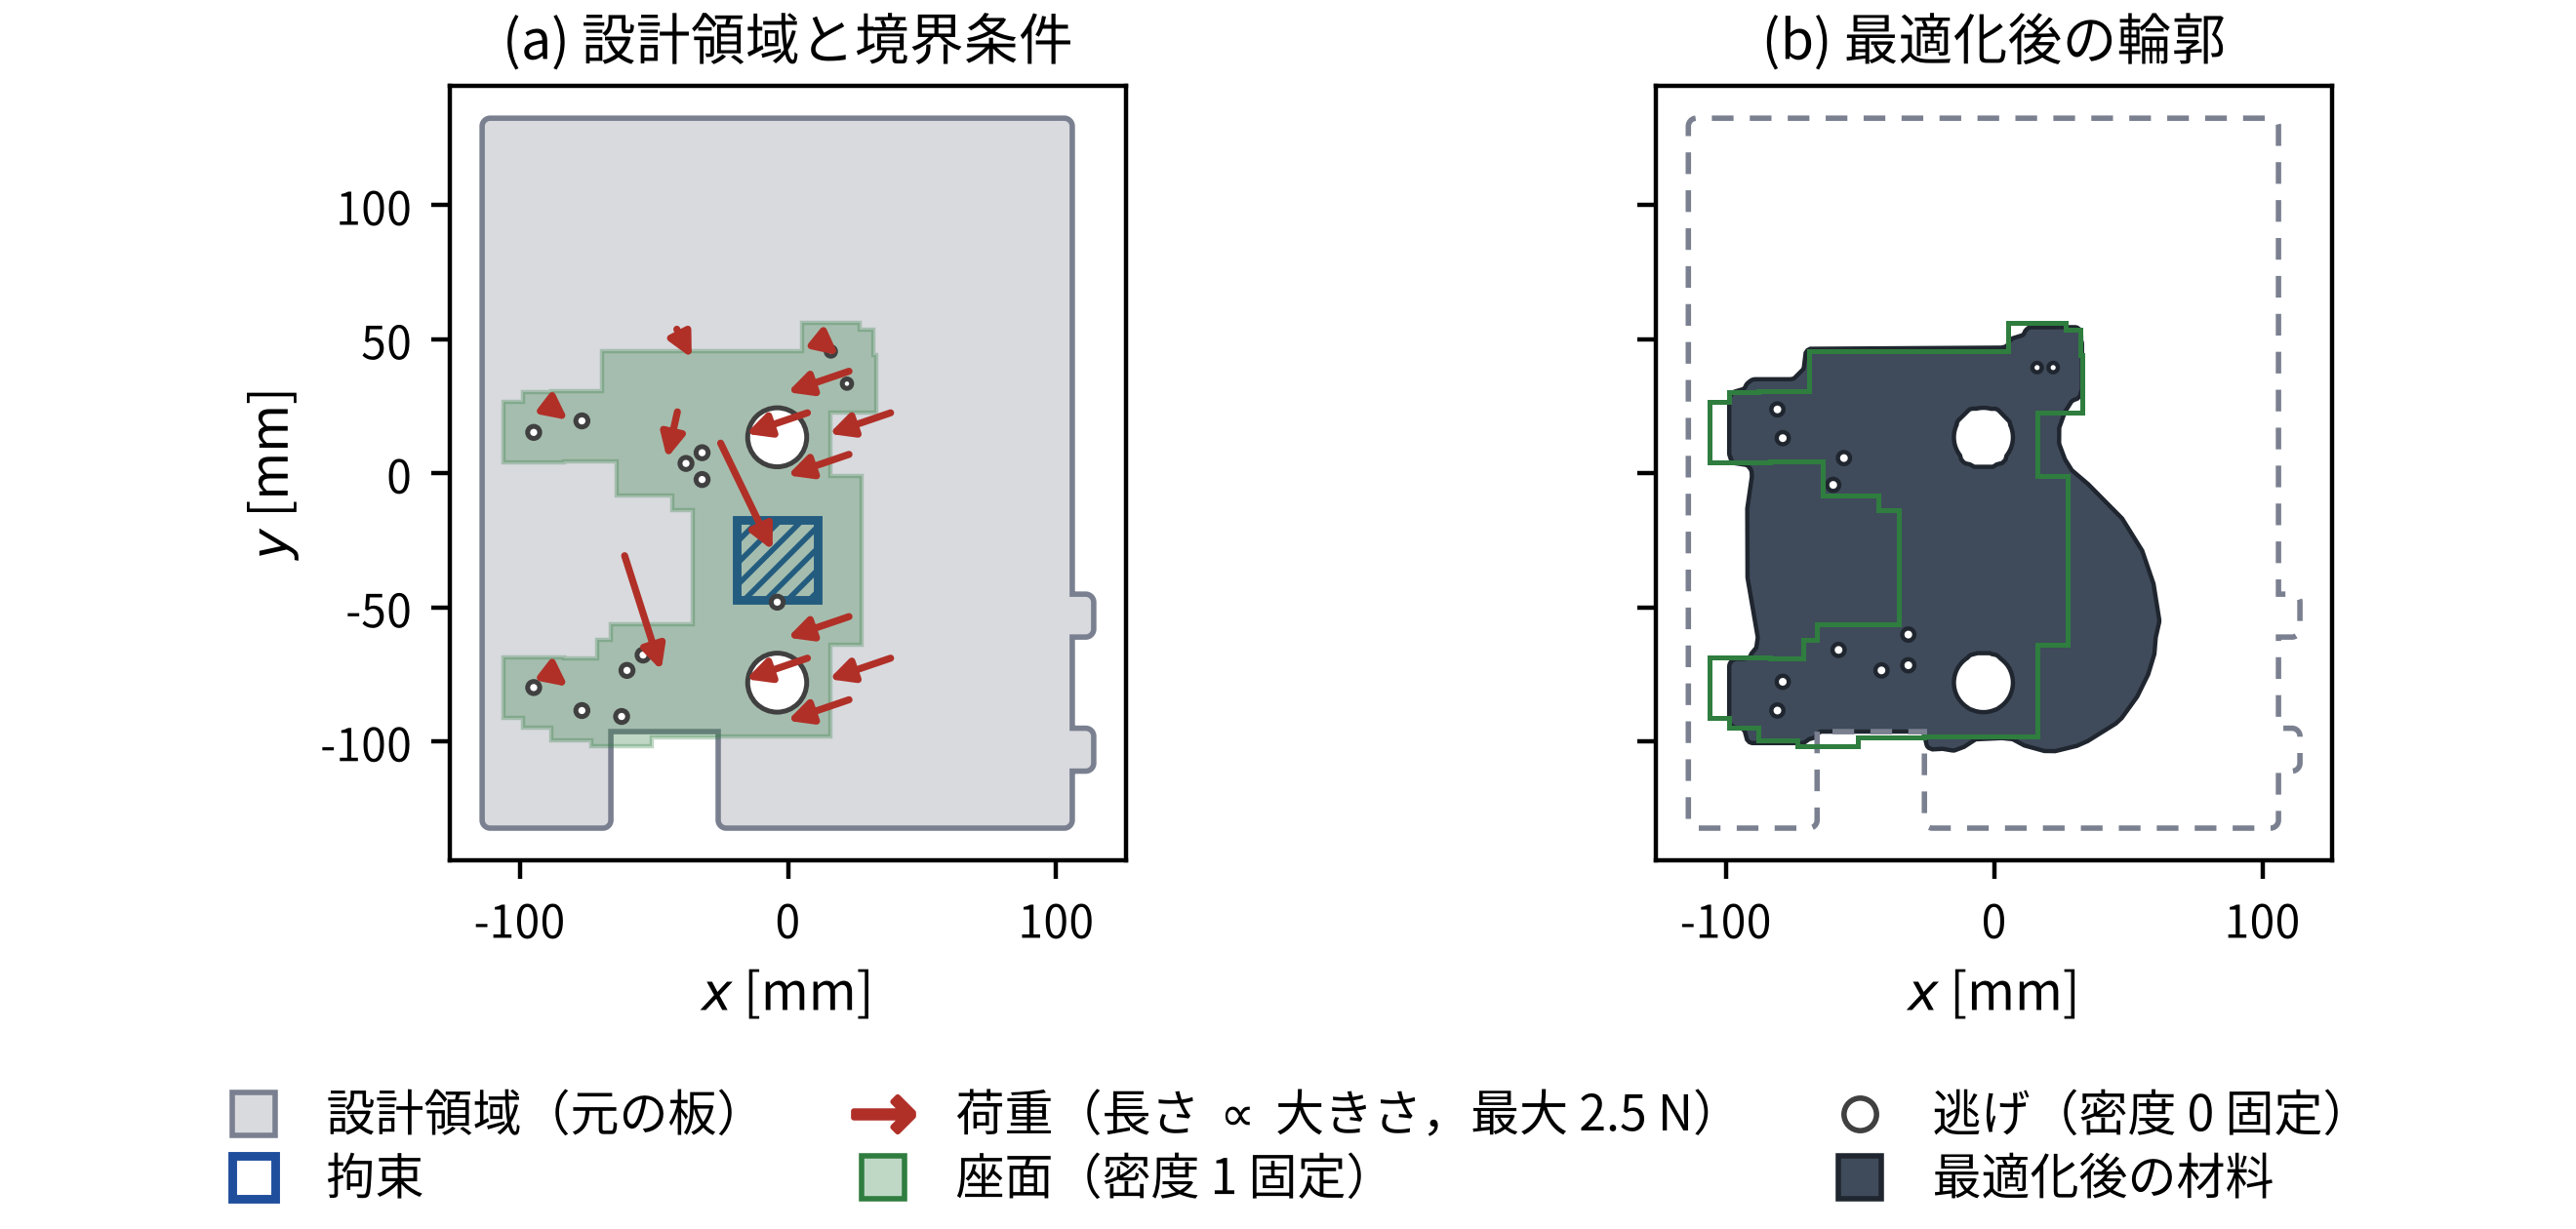
\includegraphics[width=0.86\linewidth]{figs/fig2.png}
\caption{位相最適化の入力と出力（射出ユニット側板，板厚 $3\mm$，A5052）。
(a) の境界条件は固定宣言の向きから生成したもので，手書きではない。
矢印は荷重の作用位置と向き（大きさは長さで表す）。
(b) の破線は (a) の設計領域。
体積率 $32\,\%$，最小部材幅 $11.0\mm$，質量 $372.5\to155.1\,$g。}
\label{fig:topo}
\end{figure}

%----------------------------------------------------------------------
\begin{figure}[b]
\centering
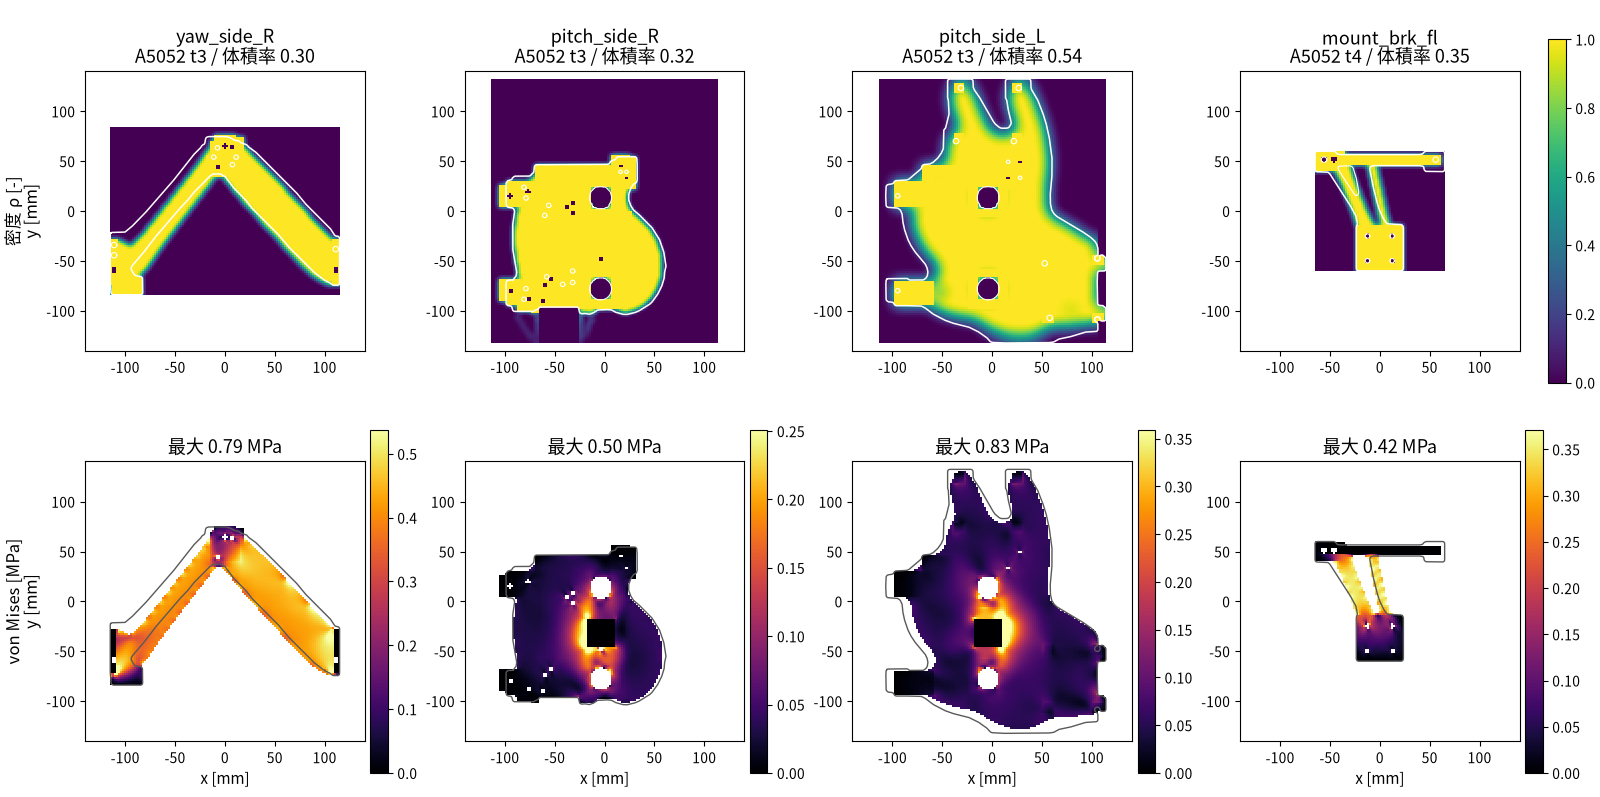
\includegraphics[width=0.72\linewidth]{figs/heat.png}
\caption{4 枚の板の密度場（上段）と von Mises 応力（下段）。
細線は実際に部品となった輪郭。応力のスケールは板ごとに異なり，
荷重は自重と横加速度のみなので絶対値の評価ではない
（A5052 の許容応力は $90\,$MPa 級）。}
\label{fig:heat}
\end{figure}

%----------------------------------------------------------------------
\begin{figure}[b]
\centering
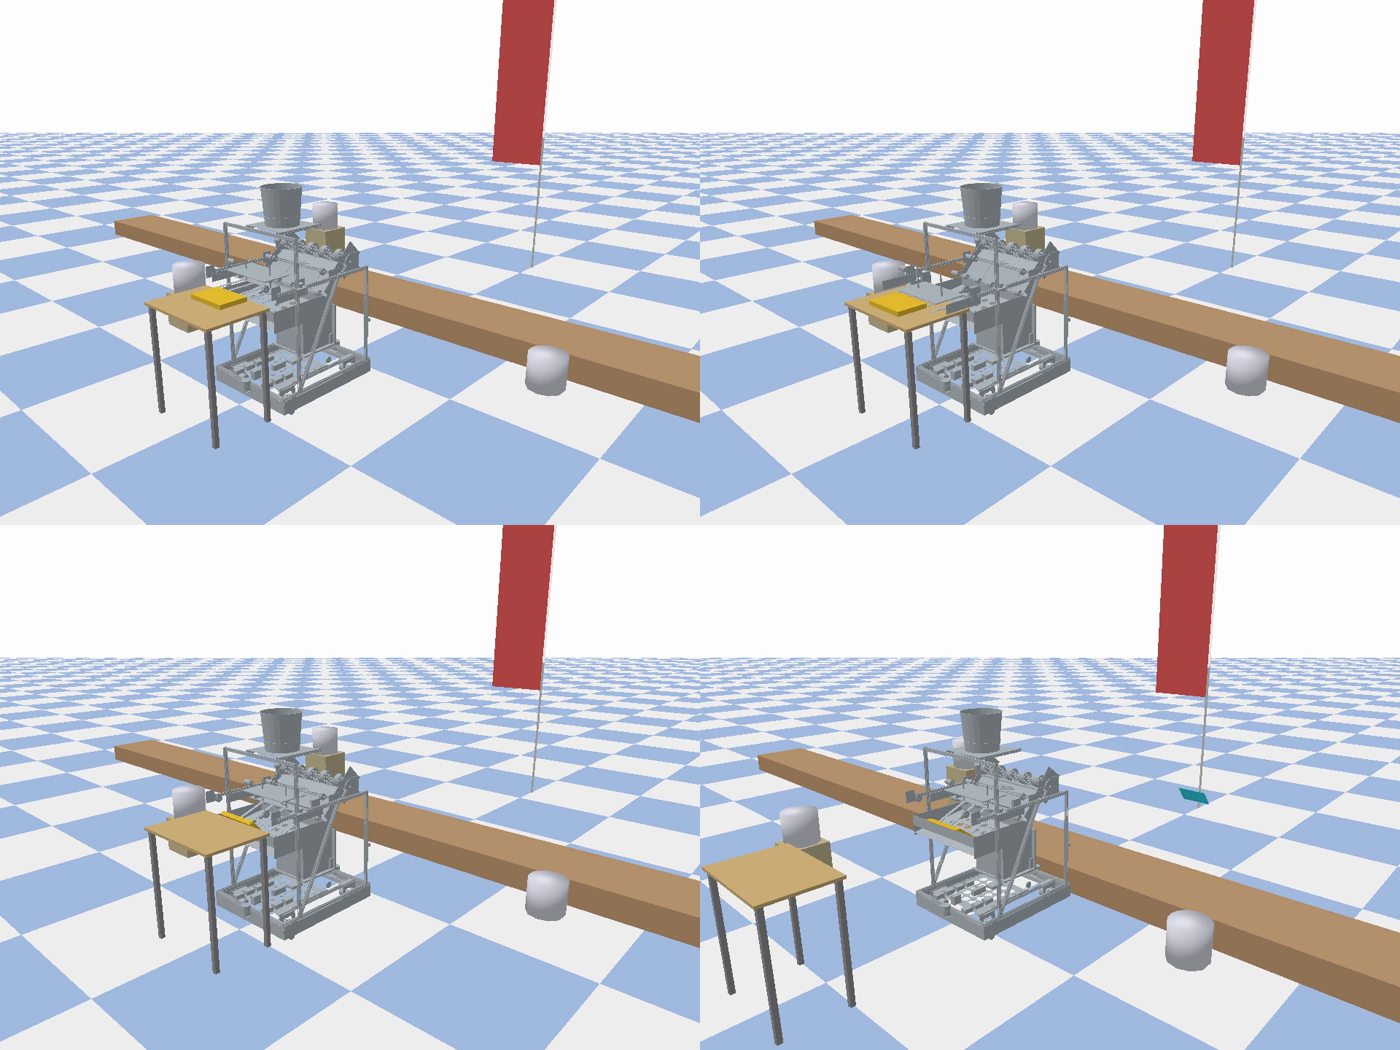
\includegraphics[width=0.62\linewidth]{figs/frames.png}
\caption{機構シミュレーション。左上から順に，接近，挿入と引込，前進，射出。
机への接触は 0 回である。この検証系に故意に旧形状を戻すと，
同一条件で接触が 884 回に転じる（4 章，様式 1 の確認）。}
\label{fig:sim}
\end{figure}


%----------------------------------------------------------------------
\section{考察: 失敗様式の類型化}

観測された不良は設計対象に固有ではなく，
表\ref{tab:modes}の六様式に帰着した。

\begin{table}[t]
\centering\footnotesize
\caption{設計自動化における失敗様式と対策}
\label{tab:modes}
\begin{tabular}{@{}p{0.33\linewidth}p{0.60\linewidth}@{}}
\toprule
様式 & 対策\\
\midrule
1. 検査の不作動 & 故意に不良を導入し，不合格になることを確認する\\
2. 代表姿勢基準 & 逃げ量は掃引包絡から逆算する\\
3. 幾何の代理の実体視 & 実体の内点判定で測る。代理が不適な相手は配置側が真値を宣言する\\
4. 生成物の相互依存 & 順序を固定して複数巡回す。据置条件と書込停止条件を分離する\\
5. 数値定義の未確認 & 値の定義を確認する前に解釈を構築しない\\
6. 偽陽性の放置 & 閾値を緩めず測り方を変える\\
\bottomrule
\end{tabular}
\end{table}

最も重大なのは様式 1 である。形状ライブラリの子ノードが親の座標変換を
保持しないため，可動部が関与する干渉判定は常に「干渉なし」を返していた。
この検査が機能した瞬間に，前章の組立不能な形状 5 件が露出した。

対策として，衝突形状に故意に不良を戻して検証した（図\ref{fig:sim}）。
旧形状では接触 0 回（検出できていない），新形状では 884 回，修正後は 0 回。
中間の結果が，検査が機能していることの証拠となる。
すなわち，検査が合格することと，検査が機能していることは別である。

様式 3 では，バウンディングボックスを実体の代理として扱った箇所が
例外なく破綻した。斜材の代理を座面としたためガセットの $60\,\%$ が
保存領域となり，「削減不能」という誤った結論を与えた例がある。
様式 6 では，ある検査が 334 件を出力したがその大半は偽陽性であり，
これが当該検査を機能停止させた。閾値を緩めるのではなく測り方を変える。

%----------------------------------------------------------------------
\section{結言}

設計妥当性を 34 系統の自動検査で判定する設計法を実機規模の機体に適用し，
図面の目視では検出し得ない不良を六つの失敗様式に類型化した。
設計の品質は作図の丁寧さではなく，何を機械的に問い続けたかで決まる。
検査は，故意の不良に対して不合格となることを確認して初めて信頼できる。

\end{document}
